 \documentclass[12pt,titlepage]{article}

\usepackage{graphics}
\usepackage{pdflscape}
\usepackage[hyphens]{url}
\usepackage{float}
\usepackage{array}
\usepackage{color}
\usepackage{colortbl}
\usepackage{xcolor}
\usepackage{url,amsfonts,epsfig}
\usepackage[applemac]{inputenc} %comando per le lettere accentate se usate mac  
%\usepackage[T1]{fontenc}
%\usepackage[utf8]{inputenc}
\usepackage[english]{babel}
%\usepackage[latin1]{inputenc} % comando per le lettere accentate se usate pc  
\usepackage[pagebackref]{hyperref}
\hypersetup{
colorlinks=false,
allbordercolors=white
}

\usepackage{listings} 
\usepackage{color} 
 
\definecolor{dkgreen}{rgb}{0,0.6,0} 
\definecolor{gray}{rgb}{0.5,0.5,0.5} 
\definecolor{mauve}{rgb}{0.58,0,0.82} 
 
\lstset{frame=none, 
  language=Java, 
  aboveskip=3mm, 
  belowskip=3mm, 
  showstringspaces=false, 
  columns=flexible, 
  basicstyle={\small\ttfamily}, 
  numbers=none, 
  numberstyle=\tiny\color{gray}, 
  keywordstyle=\color{blue}, 
  commentstyle=\color{dkgreen}, 
  stringstyle=\color{mauve}, 
  breaklines=true, 
  breakatwhitespace=true, 
  tabsize=3 
} 

\begin{document}

%Code for title page
\begin{titlepage}
\centering
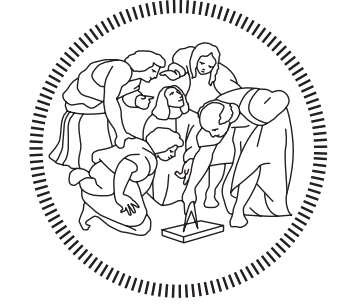
\includegraphics[width=0.4\textwidth]{Logos/LogoPolimi}\par
	{{Politecnico di Milano} \par}
	{{A.A. 2017/2018} \par}
	\vspace{1.5cm}
	
\includegraphics[width=0.9\textwidth]{Logos/LogoTravlendar}\par
	%{\Large{\textsc{{{\color{red}{ \textbf{T}rav}}lendar{\color{red}{+}}}} \\ 
		%Software Engineering 2} \par}f
	\vspace{1.5cm}
	{\Huge \textbf {DD}\par}
	{ \textbf{Design Document} \par}
	\vspace{1.5cm}
	{\Large\itshape Sara Pid\'o  }{\Large   {  894744}\par}
	{\Large\itshape Chiara Plizzari }{\Large   {  893901}\par}
	{\Large\itshape Giuseppe Severino }{\Large   {  898458}\par}
	\vspace{2cm}
	\vfill
	% Bottom of the page
	%{\large Document version: 3.1\par}
\end{titlepage}

\newpage\null\thispagestyle{empty}\newpage

\pagenumbering{roman}

%%%% Opzione per interlinea 2
%%%\baselineskip 18pt

%\maketitle

\tableofcontents
%%\listoffigures
%%\listoftables

\pagebreak

\section{Introduction} \label{introduzione}
\pagenumbering{arabic}
\subsection{Purpose}
With the Design Document we would like to make the idea of Travlendar+ application more precise and more detailed.
In particular the main goal of the DD is  to describe the system in terms of architectural design choices.
It is written in particular for developers to help them to identify the architectural styles, the design patterns, the main components and their interfaces and, last but not least, the runtime behaviour.


\subsection{Scope}
The system aims to provide a complete calendar to users which are also helped to find the best route to reach their meetings and their appointments. 
Users can insert their meetings in order to have an agenda organized in a perfect way: they can see their trips of the day, their itineraries between appointments. Users can choose between different travel options basing on distances, travel time, cost.
The system provides some features to personalize the application in order to please users. In fact they can specify lunch time, they can activate or deactivate some travel means, they can also  choose for instance to minimize the walking distance or the carbon footprint. 
With this new application, people and their smartphones can have a lot of appointments in different locations without having the concern about plan the way to reach them. Obviously if two meetings overlap or if it is not possible to reach one, the system will advice users.

\subsection{Definitions, Acronyms, Abbreviations}
\subsubsection{Definitions} 
\begin{itemize}
\item Visitor: a person that is not registered yet, but has the access to the application's information.
\item Registered user: a person that is logged in the system and can create meetings.
\item Activity: an event that happens in the real world and that could be a meeting or a break.
\item Meeting: an activity among the registered user and other people. It can be created, modified and deleted by the meeting's creator.
\item Break: an activity that a registered user can insert in order to manage it in a customizable way.
\item Trip: it indicates the route and the travel means chosen, based on user's preferences.
\item Location: fixed place where a user stands or where he/she has to attend a meeting.
\item Global preferences: they are global attributes that registered users can modify and those are valid for all trips (i.e. minimize carbon footprint).
\item Creation screen: the screen of the application in which the registered user create a meeting or a break and enters its related details.
\item Blocked travel means: it is a travel means that the user has selected as unwanted.
\item Warning: a message directed to the user that arrives to him in form of a notification and can be shown on the application screen. It is generated by the system when there are some impediments for a trip (bad weather, strikes, traffic...) or when there are some problems (invalid data during the registration process or during the creation of an activity etc...).
\end{itemize}
\subsubsection{Acronyms}
\begin{itemize}
\item DD: design document;
\item RASD: requirements analysis and specification document;
\item API: application programming interface;
\end{itemize}
\subsubsection{Abbreviations}
\begin{itemize}
\item	Gi: i-goal
\item	Ri: i-requirement
\end{itemize}
\subsection{Revision history}
This is the first version of the DD document.
\subsection{Reference Documents}
\begin{itemize}
\item RASD;
\item Specification Document;
\item Example of DD of previous years;
\item \url{https://msdn.microsoft.com/it-it/library/windows/desktop/ms685068(v=vs.85).aspx} (To describe the three tier architecture);
\item \url{https://www.alertra.com/blog/2010/improve-availability-performance-using-database-replication
} (To describe the database replication process);
\item \url{https://docs.oracle.com/cd/B14117_01/server.101/b10743/security.htm} (To describe some non functional requirements);
\item \url{https://www.tutorialspoint.com/software_testing_dictionary/thread_testing.htm} (To understand the thread testing procedure);
\item \url{https://en.wikipedia.org/wiki/Risk-based_testing} (To understand the risk-based testing procedure);
\end{itemize}
\subsection{Document Structure}
This document is structured as follows:
\paragraph{Section 1: Introduction}
In this section it is described the purpose and the main goals  of the document giving a general description.
\paragraph{Section 2: Architectural Design}
It gives a general view on how the architecture of Travlendar+ should be showing architectural choices, styles and patterns.
\paragraph{Section 3: Algorithm Design}
In this part we include the most critical and relevant parts via algorithms.
\paragraph{Section 4: User Interface Design}
This section provides an overview on how the user will see the application through the mockups and UX and BCE diagrams.
\paragraph{Section 5: Requirements Traceability}
It explains how requirements defined in the RASD must be mapped to the design elements of the application.
\paragraph{Section 6: Implementation, Integration and Test Plan}
This part will include the order of implementation of subcomponents and to integrate them. Moreover it will include our plan to test this integration.
\paragraph{Section 7: Effort spent}
Here are reported the information about the hours of work spent by each member of the group by doing this project.
\paragraph{Section 8: References}

\section{Architectural Design}
\subsection{Overview}
This section deals with the architecture of Travlendar+. It is written to explain architectural choices made for the system. These decisions are supported by different diagrams to highlight the view of components and their interactions and to clarify architectural styles adopted in a better way.

The most suitable system architecture that will allow to satisfy all requirements is a three tier architecture. It is helpful also because allows any of the three tiers to be upgraded or replaced independently in response to changes in requirements or technology.
In this pattern, we have three subsystems to decouple logic and data, logic and presentation: 
\begin{itemize}
\item Presentation layer: it is the topmost level of the application. It provides a graphic user interface to the client and it communicates with other levels by which it puts out the results to the client displaying information  related to the services and also acquires its inputs to send to other tiers.
\item Application layer:  it is the mid level. It controls Travlendar+'s functionalities by performing detailed computation. It coordinates the application, processes commands, makes logical decisions and evaluations and perform calculations. This layer also interacts with external systems that support our application.
\item Data layer: it is the level in which information are stored and managed. It includes the data persistence mechanisms (database servers, file shares etc.) and the data access layer that encapsulates the persistence mechanism and exposes the data. It is kept independent from application logic and presentation layer.
\end{itemize}

\includegraphics[scale=0.5]{"Diagrams/General Architecture - Page 1"}
\pagebreak


\subsection{Component View}
In this section we will present the whole system. We will focus on all components and their interactions. This diagram will provide also an overview on interfaces that components provide for interactions.
\begin{figure}[H]
\centering
\makebox[\textwidth]{\includegraphics[scale=0.22]{"Diagrams/Component Diagram - Page 1"}}
\caption{Entity-Relation diagram}
\end{figure}

\clearpage
\newpage

\begin{flushleft}
\begin{itemize}
\item \textbf{Event listener:} it manages the information that it receives from the user application and it sends it to the different components of our application. It decides where the information must be directed. Moreover the event listener forwards the information to the user application.
\item \textbf{Notification controller:} it manages the warnings, it creates them thanks to the trip controller and sends them to it that will show them to the user.
\item \textbf{Trip controller:} it occupies of organizing trips between activities. It uses data of the activity controller and it activates the notification controller. It exploits information of the map controller and of the external services controller (such as weather, traffic, strikes).
\item \textbf{Activity controller:} it receives information from the user to create meetings, modify them and delete them. It receives also data to create, modify and delete breaks. It gives data to the trip controller so that it can organize journeys between them.
\item \textbf{Map controller:} it gives the opportunity to the user to see information about trips that he/she has to do showing trips on the map. It visualize the daily trip between activities through data of the trip controller.
\item \textbf{External services controller:} it manages every external service exploited by our application. It receives information from them and it uses them to provide all functionalities of Travlendar+.
\item \textbf{User controller:} it manages the information about the user. It receives:
\begin{itemize}
\item personal information such that name, surname, address;
\item data for the login (username and password);
\item global preferences, for example activation or deactivation of travel means or minimum duration of the lunch break.
\end{itemize} 
\item \textbf{Model:} it is our representation of the world. It contains all data with Travlendar+ deals with.
\item \textbf{Physical Database:} it is the database to store data persistently.
\item \textbf{Web service Database:} it permits to retrieve data from the physical database using standard web service protocols.
\item \textbf{Push notification service:} it manages the sending of all notification to users' devices.
\item \textbf{Map service:} it provides the map and services like computation of trip distances and travel time
\item \textbf{External services:} they provides information and functionalities to our application. Travlendar+ exploits data like traffic, strikes, weather and it uses external applications like Ofo, Enjoy, Trenitalia to provide for example the purchase of tickets and the rent of sharing system vehicles.
\item \textbf{User application: } it is the GUI. It provides the graphic user interface to the client and communicates with the server.
\end{itemize}
\end{flushleft}

\clearpage
\newpage

\begin{landscape}
\subsubsection{Database}
The DB component will include a DBMS to properly manage the data and their handling. It will interact only with the application server. It will use a secure interface so that the date are safely stored and the security is guaranteed.
We show the data representation with  E-R schema.
\begin{figure}[H]
\centering
\makebox[\textwidth]{\includegraphics[scale=0.27]{"Diagrams/ER "}}
\caption{Entity-Relation diagram}
\end{figure}
\end{landscape}
\clearpage
\newpage

\subsection{Deployment View}
\begin{figure}[H]
\centering
\makebox[\textwidth]{\includegraphics[scale=0.4]{"Diagrams/Deployment Diagram"}}
\caption{Entity-Relation diagram}
\end{figure}

In  this section we want to show the deployment of our application showing the physical structure of the system.
We will use two servers, one for the application and the other for the data. We do not specify the type of the server to use but it should be powerful enough to support all data and all requests that there will be.

The application server will run on the execution environment JavaEE and communication with the database are possible thanks to Java Persistence API which will wrap all database functionalities.
The application server will handle all the logic behind the system.

The database server will run on the DBMS with the software MySQL. We will choose this software because it is reliable and moreover it is widely spread because it is free. This server communicates only with the application server.

Clients can use application through smartphones or tablets. The application will communicate with the application server in a direct way.

\clearpage
\newpage

\subsection{Runtime View}
We would like to show the behaviour of the application for some of the most important features: through sequence diagrams we explain how the requests of a user are managed by components of Travlendar+.

We think that the behaviour of Travlendar+ is interesting in particular for these functionalities:
\begin{itemize}
\item registration;
\item login;
\item creation of an activity;
\item modification of an activity;
\item elimination of an activity;
\item choice of a trip;
\item modification of user's preferences.
\end{itemize}

We represent the actor that initializes a process and all components of the application and entities of the database that manage to complete the requested functionality.

\begin{figure}
\paragraph{Registration}
\centering
\makebox[\textwidth]{\includegraphics[scale=0.3]{"Diagrams/Sequence Registration"}}
\caption{Sequence diagram of the registration process}
\end{figure}

\begin{figure}
\paragraph{Login}
\centering
\makebox[\textwidth]{\includegraphics[scale=0.3]{"Diagrams/Sequence Login"} } 
\caption{Sequence diagram of the login process}
\end{figure}

\begin{figure}
\paragraph{Create an activity}
\centering
\makebox[\textwidth]{\includegraphics[scale=0.2]{"Diagrams/Sequence createActivity"} } 
\caption{Sequence diagram of the creation of an activity}
\end{figure}

\begin{figure}
\paragraph{Modify an activity}
\centering
\makebox[\textwidth]{\includegraphics[scale=0.2]{"Diagrams/Sequence modifyActivity"} } 
\caption{Sequence diagram of the modification of an activity}
\end{figure}

\begin{figure}
\paragraph{Delete an activity}
\centering
\makebox[\textwidth]{\includegraphics[scale=0.28]{"Diagrams/Sequence deleteActivity"} } 
\caption{Sequence diagram of elimination of an activity}
\end{figure}

\begin{figure}
\paragraph{Choose the favourite trip}
\centering
\makebox[\textwidth]{\includegraphics[scale=0.38]{"Diagrams/Sequence chooseFavouriteTrip"} }
\caption{Sequence diagram of choosing the trip}
\end{figure}
\clearpage
\newpage

\begin{figure}
\paragraph{Modify user's preferences}
\centering
\makebox[\textwidth]{\includegraphics[scale=0.4]{"Diagrams/Sequence ModifyUserPreferences"}  }
\caption{Sequence diagram of modifying user's preferences}
\end{figure}

\clearpage
\newpage


\begin{figure}
\subsection{Component Interfaces}
\centering
\makebox[\textwidth]{\includegraphics[scale=0.6]{"Diagrams/Components interfaces"}  }
\end{figure}
\clearpage
\newpage
\subsection{Selected Architectural Styles and Patterns}
\subsubsection{Three-Tier Architecture} 
As we said before the architectural style that we have chosen for our application is a standard three-tier architecture. The tiers are the following:
\begin{itemize}


\item[1] GUI Tier: Thin clients. They display information and make the different services and functionalities reachable from the client. Clients can communicate with other tiers.
\item[2] Application Tier: It controls application functionality, manages requests coming from the clients and sends results, data and notifications to them. It retrieves data from the Data Tier.
\item[3] Database Tier: Houses database servers where information is stored and retrieved. Data in this tier is kept independent of application servers.
\end{itemize}
We choose this type of architecture because it has proved to be effective. It allows a developer the opportunity to extend, modularize, and be able to configure their application.
Here we list 5 benefits of separating an application into three different tiers:
\begin{itemize}
\item[1] It gives you the ability to update the technology stack of one tier, without impacting other areas of the application.
\item[2] It allows for different development teams to each work on their own areas of expertise.
\item[3] You are able to scale the application up and out, e.g. you can use different technologies to deploy database instead of being stack with only one.
\item[4] It adds reliability and more independence of the underlying servers or services.
\item[5] It provides an ease of maintenance of the code base, managing presentation code and business logic separately.
\end{itemize}
Moreover with three-tier architecture there is the possibility to use new technologies as soon as they become available. This ensures the product is ready to adapt. There is the possibility to redesign your product.
\subsubsection{Design Pattern}
\paragraph{Client Server}
The application is designed to follow the Client-Server communication model. Travlendar+ should be distributed, reachable from a large number of different devices and it needs to provide the service to all of them.
We would like to have thin clients: we design the server to manage requests and data, while the client should only see results and provides the user with the possibility of exploiting every functionality that they can use.
Moreover the client-server model allows our system to have high maintainability and scalability.


\paragraph{MVC Pattern} The application follow the Model-View-Controller software design pattern. This allows our application to be separated into three communicating parts.
\begin{itemize}
\item The model represents only the data and nothing else. It does not depend on the controller or on the view.
\item The controller provides model data to the view and receives user actions from the view. It depends on the other two parts.
\item The view displays the data and sends user actions to the controller.
\end{itemize}
We choose to use this pattern for different reasons: it fits very well with three-tier architecture, it guarantees more reusability to our application and it provides modularity.

\section{Algorithm Design}
In this section we highlight some of the algorithms used for the implementation of the critical part of our application. In particular, the following are the algorithms used for deploying the application in Android (developed using Java language). 
\subsection{Adding an activity} 
In this piece of code is shown the function called by the event listener when a registered user insert a new activity (meeting or break) in Travlendar+. It calls the function \textit{checkWarning} from the class \textit{NotificationController} that will be explained in the next subsection. 
\begin{lstlisting} 
public class ActivityController { 
  //Add a new activity to an existing trip 
  public void addActivity(RegisteredUser ru, Activity a) 
  { 
    if (ru.getCalendar().getTrips().getTrip(a.getData()) != null) 
        //Create a new trip with the same data of the activity 
        ru.calendar().getTrips().createTrip(a.getData());  
    //Get the existing trip with the same data of the activity 
    Trip currentTrip = ru.getCalendar().getTrips().getTrip(a.getData());  
    currentTrip.add(a); 
    orderActivities(currentTrip); 
    //If there are some errors, delete the activity from the user's trip 
    if (NotificationController.checkWarning(currentTrip)=true)  
      currentTrip.remove(a); 
    else  
      { 
        //Compute and show to the user the path's alternatives to reach the meeting 
        TripController.computeTripPath(currentTrip);  
      } 
  } 
   
  //Insertion sort algorithm based on the starting time of activities in the trip (converted in minutes for the sake of semplicity) 
  private void orderActivities(Trip t)  
  { 
    int i, j; 
    for(i=1; i<t.length(); i++) 
    { 
      int tmp = convertToMinutes(t.get(i).getTime().getHour(), t.get(i).getTime().getMinute()); 
      for (j = i - 1; (j >= 0) && (convertToMinutes(t.get(j).getTime().getHour(), t.get(j).getTime().getMinute()) > tmp); j--)  
      { 
              t.get(j + 1) = t.get(j); 
               
          } 
       
      t.get(j + 1) = tmp; 
    } 
  } 
   
  //Utility function that express a time in its equivalent in minutes  
  private int convertToMinutes(int hour, int minutes) 
  { 
    return hour*60+minutes; 
  } 
  ... //Other functions 
} 
 
 
public class TripController { 
 
  public void computeTripPath(RegisteredUser ru, Trip t) 
  { 
    //Call external services to generate various path alternatives (and by using the trip preferences specified by the user) 
    ExternalServicesManager.computePath(t); 
    //Show the generated alternatives to the user 
    ru.show(t.getPathAlternatives());  
  } 
  ... //Other functions  
} 
\end{lstlisting} 
 
\subsection{Notification Controller} 
Below is provided the implementation of the checks that are performed when a new activity is added to an existing trip. When a check returns false, then a warning is generated and it will appear as pop-up notification in the user's device, by invoking the \textit{sendWarning()} function. 
\begin{lstlisting} 
public static class NotificationController { 
   
  public static boolean checkWarning(Trip t) 
  { 
    boolean error = false; 
    if (overlappingActivities(t))  
    {   
      //Create a new warning by specifying (type, description) 
      Warning warning = new Warning("OverlappingActivities", "Two activities overlap");  
      //Activate the function that will send the notification to the user's device 
      warning.sendWarning(); 
      error = true; 
    } 
    if (activityUnreachable(t))  
    {   
      //Create a new warning by specifying (type, description) 
      Warning warning = new Warning("ActivityUnreachable", "The new activity make the next activity unreachable");  
      //Activate the function that will send the notification to the user's device 
      warning.sendWarning(); 
      error = true; 
    } 
    return error; 
  } 
   
  private static boolean overlappingActivities(Trip t) 
  { 
 
    for(int i=1; i<t.length(); i++) 
    { 
      //timeInMinutes1 expresses the activity i-1's starting hour in minutes  
      int timeInMinutes1 = convertToMinutes(t.get(i-1).getTime().getHour(), t.get(i-1).getTime().getMinute()); 
      //timeInMinutes2 expresses the activity i's starting hour in minutes  
      int timeInMinutes2 = convertToMinutes(t.get(i).getTime().getHour(), t[i].getTime().getMinute()); 
      if (timeInMinutes1+t[i-1].getDuration() > timeInMinutes2) 
        return true; 
 
    } 
    return false; 
  } 
   
  private static boolean activityUnreachable(Trip t) 
  {  //t.get(i).getTravelDuration() returns the time for moving from the activity i-1 to the activity i. 
    //It is already expressed in minutes 
 
    for(int i=1; i<t.length(); i++) 
    { 
      //timeInMinutes1 expresses the activity i-1's starting hour in minutes  
      int timeInMinutes1 = convertToMinutes(t.get(i-1).getTime().getHour(), t[i-1].getTime().getMinute()); 
      //timeInMinutes2 expresses the activity i's starting hour in minutes  
      int timeInMinutes2 = convertToMinutes(t.get(i).getTime().getHour(), t[i].getTime().getMinute()); 
       
      if (timeInMinutes1+t[i-1].getDuration()+t.get(i).getTravelDuration() > timeInMinutes2) 
        return true; 
    } 
    return false; 
  } 
  ... //Other functions 
} 
\end{lstlisting} 


\section{User Interface Design}
Mockups of Travlendar+ have already been presented in the \textit{Requirements Analysis and Specification Document} to show the look of our application. Now, we want to describe more in detail the features offered by the graphical interface and the way the user will provide inputs and see output on the different application screens.
\clearpage
\newpage

\subsection{Login and registration}\label{sec:Login}
This is the first screen of the application. It is shown to the user in one of the following cases:
\begin{itemize}
\item It's the first launch of the application on the user's device;
\item The registered user has decided to log out his/her account from the application;
\item The registered user doesn't select the \textit{Remember me} option and performs a new launch of the application.
\end{itemize}
A new user can access the registration process by pressing the \textit{Sign up}, or can access to an existing account by entering the credential in the two input form \textit{Username} and \textit{Password}. By pressing the first \textit{Login} button the user will send his/her credential to the system that will check their correctness.
\begin{figure}[H]
\centering
\makebox[\textwidth]{\includegraphics[scale=0.11]{"Mockup/mockup login"} }
\end{figure}
\clearpage
\newpage

\subsection{My activities}
This is the main screen of Travlendar+. Here is shown to the registered user a list containing all his/her activities created, divided into the two sections \textit{Meetings} and \textit{Breaks}. In the \textit{Breaks} section are also present the breaks added automatically by Travlendar+ if the user has activated, in his/her account preferences, the option for the flexible lunch. By pressing an element of the list, the user can change the activity details and can also delete it, or can press the plus symbol (see symbol no. 4) to open the Add activity's screen (see section \ref{activityScreen}).
By pressing the symbol no. 1 the user will open the application's sections list (right figure), which shows all the area of Travlendar+ application. With the two arrows present in the box no. 2 the registered user can select the day of which he/she wants to see the activities, and by pressing the current day displayed (i.e. \textit{Today}) the entire calendar will be shown. The symbol of the gear (see symbol no. 3) will open the current trip preferences.
\begin{figure}[H]
\centering
\makebox[\textwidth]{\includegraphics[scale=0.11]{"Mockup/mockup meeting"} {\includegraphics[scale=0.11]{"Mockup/mockup options"} }}
\end{figure}
\clearpage
\newpage

\subsection{Add activity and modify activity}\label{activityScreen}
Referring to the left figure, in this screen the user can specify the type of activity to add by pressing one of the three figure on the top, and then he/she must provide all the required information in order to correctly create the selected activity. By pressing the arrow on the top right, the system will compute various trip option that will be shown to user (see section \ref{trip}). 
In the right figure, instead, the user can see all the activity details, or he/she can modify an existing activity and can confirm the changes made by pressing the tick button in the upper right. He/she can also delete the activity by pressing the trash icon.
\begin{figure}[H]
\centering
\makebox[\textwidth]{\includegraphics[scale=0.11]{"Mockup/mockup add activity"} {\includegraphics[scale=0.11]{"Mockup/mockup modify activity"} }}
\end{figure}
\clearpage
\newpage

\subsection{Trip selection and trip map}\label{trip}
After the addition of a new activity, the screen present in the left figure shows to the user the various trip option computed by Travlendar+'s external services, compatibly with the user specified trip preferences. After the user selects one of the option available on the list, the right figure's screen is shown, containing the entire itinerary for the current trip. It is also shown the weather for the trip's date and the trip information such as strikes and traffic, if available. The map shows the various meetings and breaks with a blue and red signal, respectively, and by pressing the name of the activity (e.g. Take kids to school) it will enter the activity details (see section \ref{activityScreen}, right screen). By pressing the green GO button the user will be redirected to the travel instruction, while pressing the symbol with the arrow immediately below will activate the GPS service to check the current position of the user.

\begin{figure}[H]
\centering
\makebox[\textwidth]{\includegraphics[scale=0.11]{"Mockup/mockup trip selection"} {\includegraphics[scale=0.11]{"Mockup/mockup map"} }}
\end{figure}
\clearpage
\newpage

%\resizebox*{1\textwidth}{!}{
\begin{table}[ht]
\section{Requirements Traceability}

\subsection{Functional Requirements}
We describe the relationship between the requirements of Travlendar+ listed in the RASD and the components that are part of our application.
To make easier to understand, we do not list every requirement but we express the requirements in terms of the goal to which they refer.
\begin{tabular}{p{9cm}|p{5cm}}
\textbf{ Requirements of Goals} & \textbf{Components} \\ \hline
\textbf{ {[G\textsubscript{1}]}} user should be able to go to a meeting. & EventListener \linebreak ActivityController \linebreak TripController \\ \hline
\textbf{ {[G\textsubscript{2}]}} A user should be able to know if he/she cannot arrive on time to a meeting. &EventListener\linebreak ActivityController\linebreak TripController\linebreak NotificationController\\ \hline
\textbf{ {[G\textsubscript{3}]}} A user should be able to have a break that has a certain
duration between two meetings.& EventListener \linebreak ActivityController\linebreak UserController \\ \hline
\textbf{ {[G\textsubscript{4}]}} The time or the location of a meeting can be modified. &EventListener \linebreak ActivityController\linebreak MapController \linebreak  \\ \hline
\textbf{ {[G\textsubscript{5}]}} A user should be able to unsay a meeting.&EventListener \linebreak ActivityController\linebreak \\ \hline
\textbf{ {[G\textsubscript{6}]}} A user should be able to have some preferences for the trip.&EventListener \linebreak UserController\linebreak TripController \\ \hline
\textbf{ {[G\textsubscript{7}]}} A user should be able to know every possible option to go to a meeting with different travel means in order to choose the suitable one.& EventListener \linebreak TripController\linebreak MapController \\ \hline
\textbf{ {[G\textsubscript{8}]}} A user should be able to buy public transportation tickets or day/week/season pass basing on his/her needs. &EventListener \linebreak TripController\linebreak  ExternalServicesController\\ \hline
\textbf{ {[G\textsubscript{9}]}} A user would like to see on Tripadvisor advised places for
his/her breaks. &EventListener \linebreak ActivityController\linebreak ExternalServicesController \\ \hline
\textbf{ {[G\textsubscript{10}]}} A user would like to locate the nearest vehicle of a vehicle sharing system if he/she wants to use that type of travel means. &EventListener \linebreak ExternalServicesController  \\ \hline
\textbf{ {[G\textsubscript{11}]}} A user would like to have real-time news on strikes, weather
and traffic. & EventListener \linebreak  ExternalServicesController\\ \hline
\end{tabular}
\end{table}
%}

\clearpage
\newpage
\subsection{Non Functional Requirements} 
\begin{itemize}
\item \textbf{Performance} 
As already stated in the \textit{Design constraint}'s section of our RASD, the application will be developed for both Swift (for the iOs version) and Java (for the Android version) programming languages, rather than developing a single cross-platform application. This choice involves some advantages in terms of performance, including less response time and a better use of the graphics libraries belonging to each language.

\item \textbf{Availability} To ensure availability the database server and the application will be running 24 hours per day. Moreover, it is implemented the database replication capability to automatically maintain a copy of the database at a separate location. This allow the system to switch to a backup system quickly since it doesn't have to wait for a restore from tape, which could potentially take hours.

\item \textbf{Security}
To protect data exchange between the application and the server, we adopt the Hyper Text Transfer Protocol Secure (HTTPS) to encrypt all the communications and to ensure that the can not be intercepted by external subjects. 
Instead, database security is guaranteed by the implementation of a a secure authentication method for manipulating data and the use of roles and privileges, to allow or block the execution of certain queries by the user of the application.

\item \textbf{Maintainability}
System maintenance and testing are periodically performed in order to find out possible errors, security flaws or bottleneck that could affect the proper running of the application.

\end{itemize}

\pagebreak

\section{Implementation, Integration and Test Plan}
In this part we will define a plan to implement the components of Travlendar+ and to test our application and also the integration between components.
We would like to identify:
\begin{itemize}
\item objectives and scope;
\item documents and items that need to be available to perform the various quality assurance activities;
\item the order in which we will implement the subcomponents of the system;
\item the order in which we will integrate the subcomponents;
\item items and functionalities to be tested;
\item  the analysis and test activities to be performed.
\end{itemize}

\paragraph{Objectives and scope}
We want to define a plan to implement and integrate the various components of our application. We would like to test them in order to find and correct the bugs in Travlendar+ with a systematic testing.  
The scope of the implementation and integration plan described in this section is to make easier for developers to identify the optimal way to implement the application: they can easily find the most critical functionalities and the best way to integrate them with the system. Moreover they are able to organize the division of the work in an efficient way.
On the other side, the scope of the test plan is a guide line to find problems early and in an exhaustive way, to facilitate changes, to guide the design and to provide a correct modules' interactions.
\paragraph{Available documents}
To perform an implementation and an integration test plan with meaningful results, we need that the RASD is available and already completed and discussed at the point the testing will be performed. It describes the application and the functionalities of it.
Moreover it is required the DD because it provides an idea of the architecture of the system and it depicts components and their functionalities.
\subsection{Implementation and integration plan}
We will list all the functionalities with their relatives components in the order that must be followed to implement and to integrate the application.
\paragraph{Creation of the database and its web service}
The first thing to be implemented is the creation of the database that is modelled by the ER diagram and consequently the creation of the web service that relate the physical database to the application server.
\begin{figure}[H]
\centering
\makebox[\textwidth]{\includegraphics[scale=0.5]{"Diagrams/impl1"} }
\end{figure}
\paragraph{Creation and management of the trip}
One of the basic functionality that has to be implemented is the creation and the management of the trip. We will implement the creation of the activity that is followed by the creation of the daily trip. After that we will focus on the management of the trip: the user can modify activities' informations or delete them.
We will implement and integrate the activity controller, the trip controller and the calendar controller.
\begin{figure}[H]
\centering
\makebox[\textwidth]{\includegraphics[scale=0.5]{"Diagrams/impl2"} }
\end{figure}
\paragraph{Integration of the third part services}
The application uses third part services to compute the trip with different travel means and different paths. We will implement the external service by using provided APIs. We will also implement the map controller that exploits the same external application and that shows the daily trip chosen by the user.
\begin{figure}[H]
\centering
\makebox[\textwidth]{\includegraphics[scale=0.5]{"Diagrams/impl3"} }
\end{figure}
\paragraph{Management of user's account}
Travlendar+ has to manage the creation of a new user's account and also to permit to a registered user to login, eventually using pre-existent social networks' account. The component that deals with all these functionalities is the user controller. It leans on the external services controller to handle the verification of external accounts and data.
 \begin{figure}[H]
\centering
\makebox[\textwidth]{\includegraphics[scale=0.5]{"Diagrams/impl4"} }
\end{figure}
\paragraph{Management of user's preferences}
After having implementing all the basic functionalities of the application, it is necessary to add the user's preferences area. In order to do this, it is necessary to add features to the user controller. It must be able to interact with the trip controller so that the chosen trip will respect the preferences of the user.
\begin{figure}[H]
\centering
\makebox[\textwidth]{\includegraphics[scale=0.5]{"Diagrams/impl5"} }
\end{figure}
\paragraph{Additional features (notifications, weather, traffic, strikes)}
Travlendar+ must be also able to send warnings to users and inform them about the traffic, the weather or the strikes. The notification controller will be implemented and some features will be added to the external services controller.
\begin{figure}[H]
\centering
\makebox[\textwidth]{\includegraphics[scale=0.5]{"Diagrams/impl6"} }
\end{figure}
\subsection{Test plan}
In order to perform a testing activity that will guarantee the discover of bugs and the integration correctness, we chose a strategy that combines thread and critical modules integration testing. We chose to adopt this approach because we think that it's the most suitable one to test large subsystems such as Travlendar+.
In particular, with the thread approach we verify the key functional capabilities that carry out specific task. A "thread" is a portion of several modules that together provide a user-visible program feature. Threads are integrated and tested incrementally as subsystems and then performed as a a whole system.
Whereas, the critical modules integration testing consists in prioritize the tests of features and functions in software, based on the risk of failure, the function of their importance and likelihood or impact of failure. 

\pagebreak

\section{Effort Spent}
As for the RASD, we always tried to work together also for the DD. We managed to do the work in a distributed way between days. We spent about 28 hours each to write and to try to do our best for this part of the project.
We spent also other time to fix the RASD and to adjust some diagrams and some details that we thought to be wrong.

\section{References}
\begin{itemize}
\item Professor Rossi's slides;
\end{itemize}
\end{document}